% !TEX encoding = UTF-8 Unicode
\documentclass[a4paper,12pt]{article}
\usepackage{polski}
\usepackage[utf8]{inputenc}
\usepackage{graphicx}
\usepackage{float}
\usepackage{rotating}
\usepackage{caption}
\usepackage{subcaption}
\usepackage{pdfpages}
\usepackage{ucs}
\usepackage{amsmath}
\usepackage{amsfonts}
\usepackage{amssymb}
\usepackage{ucs}
\usepackage{epstopdf}
\usepackage{epsfig}
\usepackage{url}


\begin{document}
% Strona tytułowa
\begin{titlepage}
\begin{center}
\vspace*{1cm}
{ \Large \textbf{ Raport }}\\[1cm]

%{ \Large \textsc{\\ robota mobilnego} }\\[2cm]

{ \Large Projekt specjalnościowy ARR \\
\textbf{Stanowisko do badania systemu sensorycznego cybernetycznej dłoni}}\\
Semestr letni 2016/2017\\[2cm]

\Large{
\textbf{Zespół:}}\\
\large {Artur Błażejewski, 200541\\
Dawid Chechelski, 197002\\
Paweł Jachimowski, 200355\\
Krzysztof Kwieciński, 200418\\
Witold Lipieta, 200415}

\vfill
\Large
Politechnika Wrocławska\\
\large
Wydział Elektroniki\\
Automatyka i Robotyka\\
ARR
\end{center}
\end{titlepage}


	\section{Komponenty układu}
		\subsection{Cybernetyczna proteza dłoni - Grzegorz Wiśniewski}
			W projekcie czujniki zostały umieszczone na protezie skonstruowanej przez Grzegorza Wiśniewskiego. \cite{Reka}
		\subsection{Czujniki}
			W projekcie zostały wykorzystane moduły czujników stworzone przez Mariusza Głębockiego. \cite{Moduly}
			
			W modułach zostały zastosowane czujniki \cite{MPL112A2}
			
		\subsection{Płytka}
			
			\begin{figure}[H]
		     	 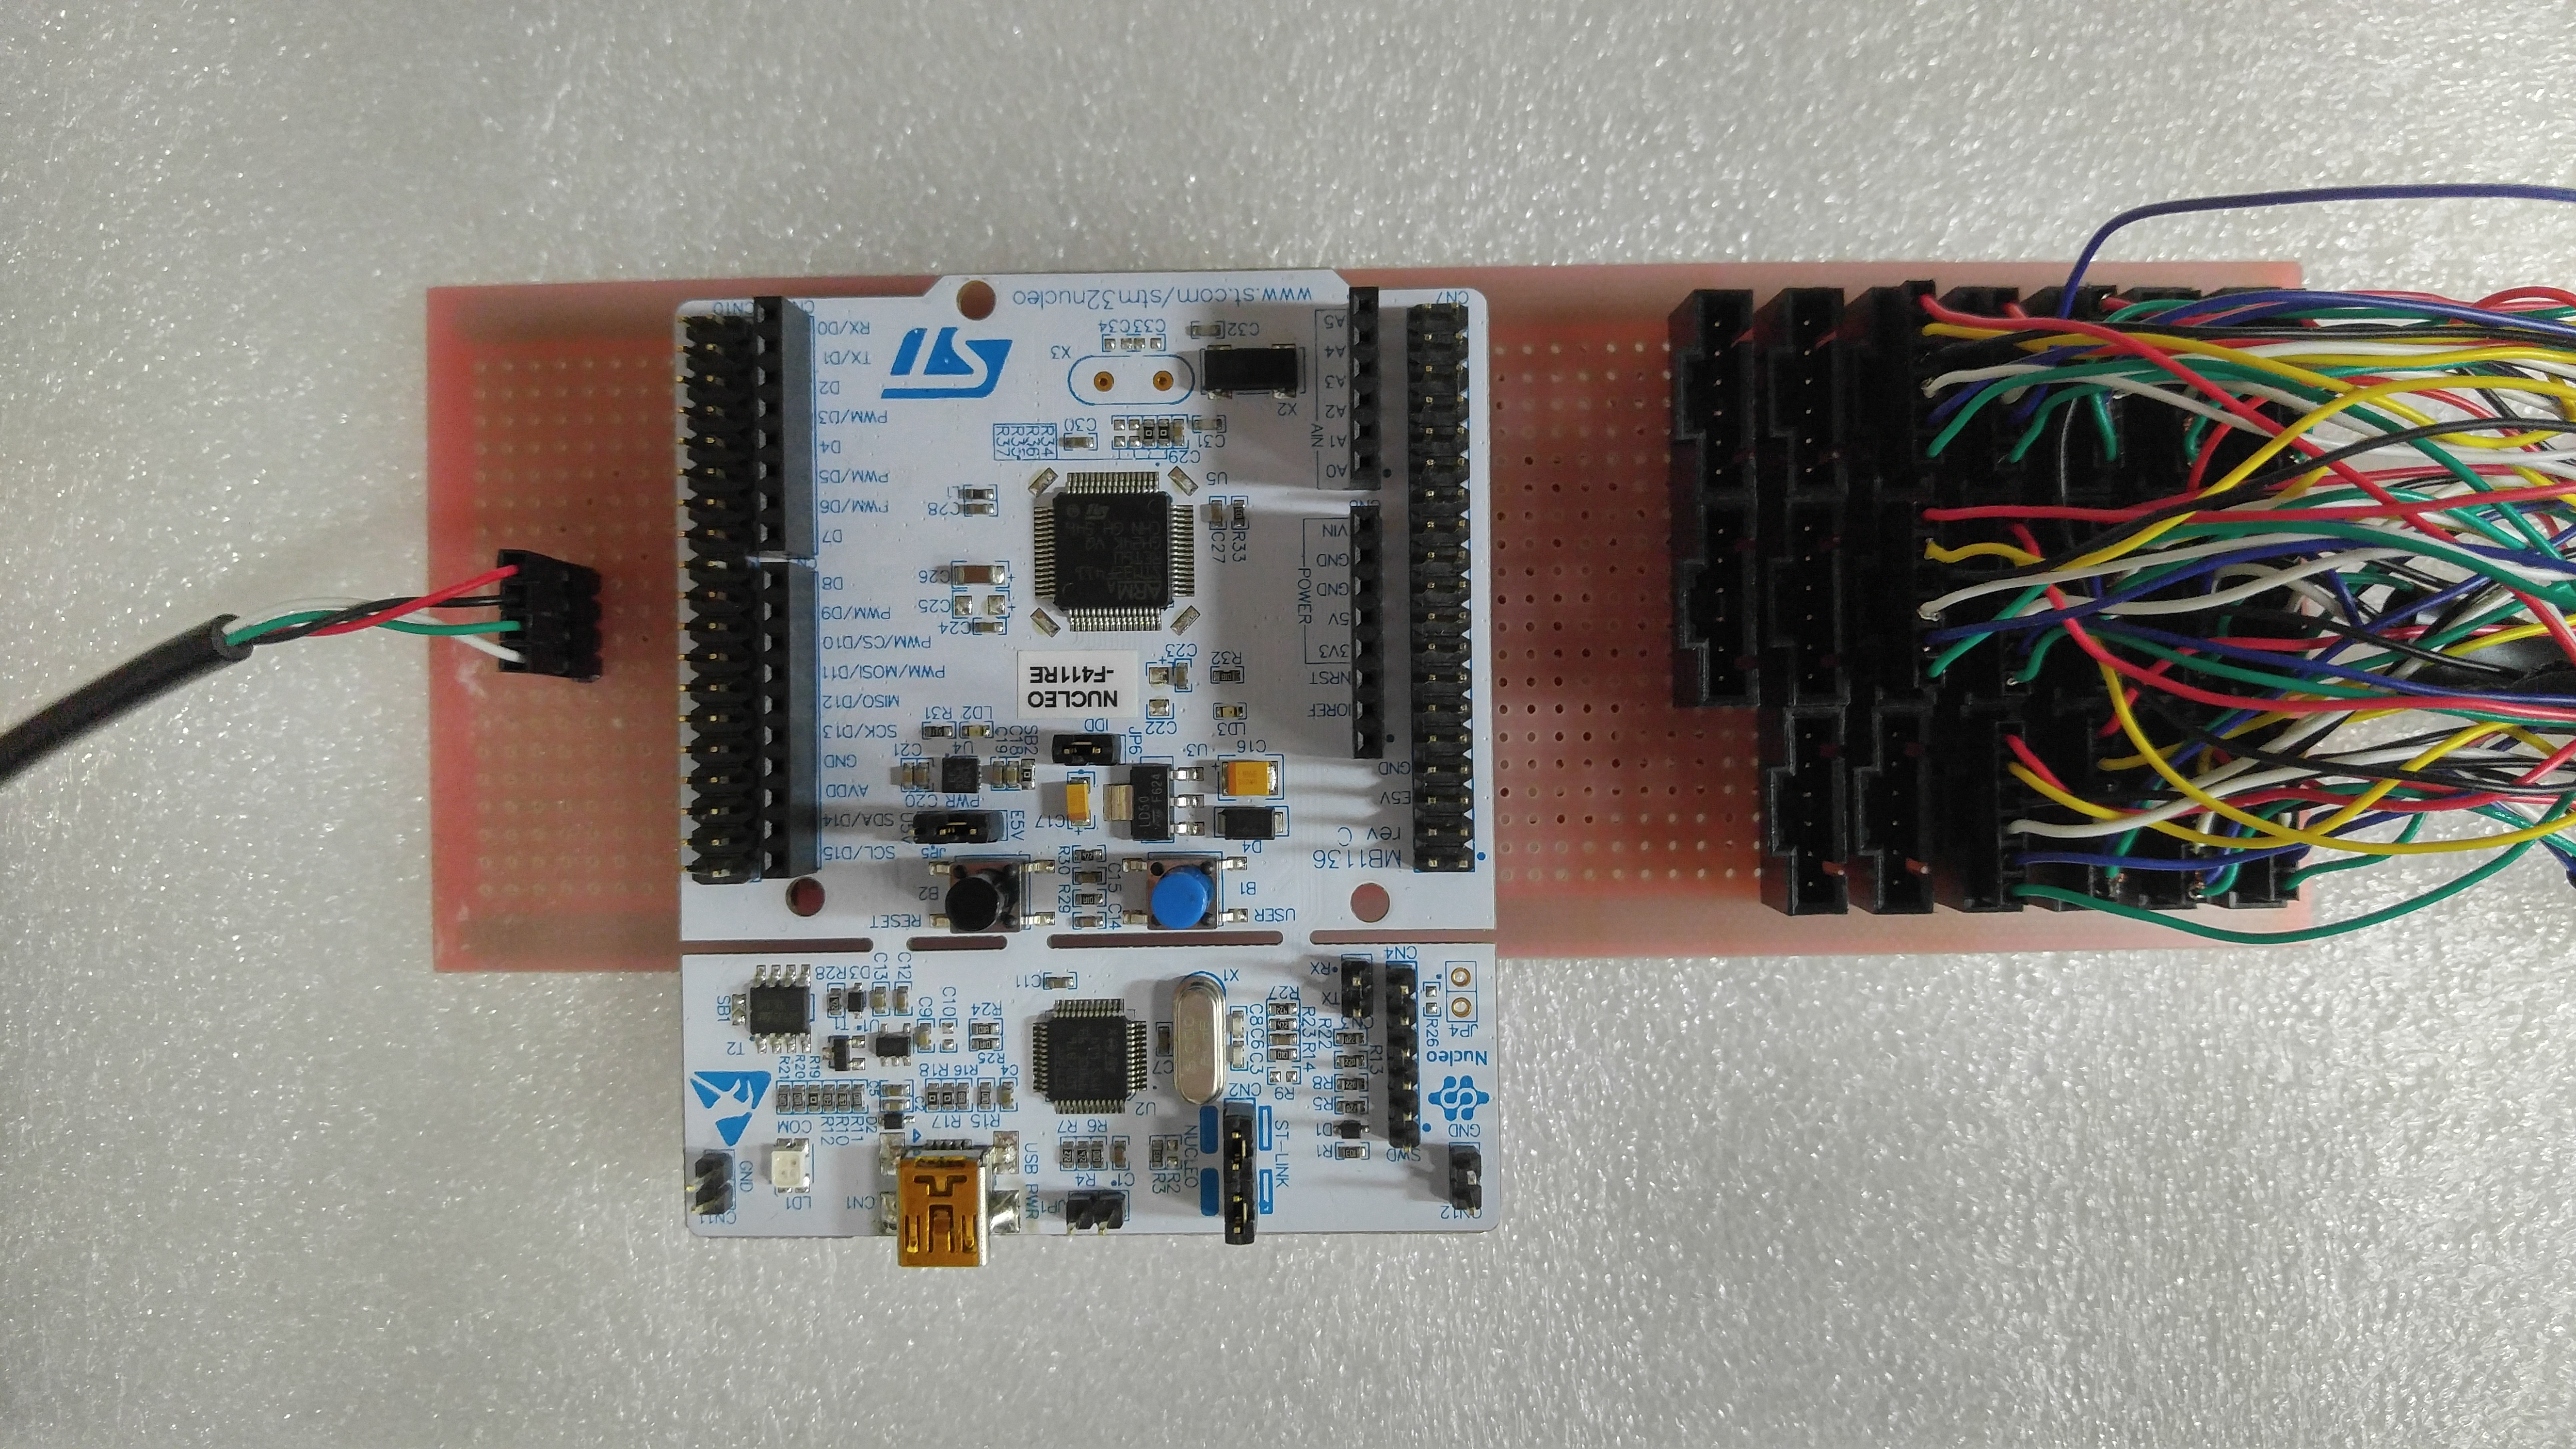
\includegraphics[width=0.1\textwidth]{obrazy/plytka.png}
			\end{figure}
		
			\subsubsection{Płytka}
				W projekcie została użyta uniwersalna płytka o wymiarach 17x6.5 cm na której zostało umieszczone 20 złącz pod czujniki oraz złącze pod komunikację uart i Nucleo. 
						
			\subsubsection{Moduł nucleo}
				Ze względu na potrzebną ilość portów komunikacji i2c wybrano moduł STM32 NUCLEO-F411RE
			
	\section{Wykonanie projektu}		
		\subsection{Komunikacja}
			\subsubsection{Czujniki}		
				Czujniki z modułem Nucleo wykorzystują komunikację i2c do połączenia, karzdy czujniki jest odpytywany osobno a następnie zebrane dane zostają przesłane do komputera.
			\subsubsection{Przesyłanie danych do komputera}
			Dane przesyłane zostaną w postaci ośmiobajtowej ramki. Pojedyńcza wiadomość będzie zawierać informację o ciśnieniu, temperaturze i identyfikator czujnika oraz bajt start, bajt sumy kontrolnej.
			\subsubsection{Komputer}
				Połączenie ręki z komputerem zostało opracowane z wykorzystaniem komunikacji UART. W tym celu skonfigurowano odpowiednie wyprowadzenia z mikrokontrolera na płytce Nucleo. Od strony komputera użyto przejściówki RS-232 na USB. Prędkość komunikacji ustawiono na 115200 bps, co wystarcza do natychmiastowego przesyłania danych z czujników.	
		\subsection{Software}
			\subsubsection{Nucleo}
				Program został napisany w języku C i źródła zostaną załączone do raportu w osobnych plikach.
			\subsubsection{Wizualizacja}
				Część wizualizacyjna została napisana w języku C++ i bibliotekach Qt. Źródła projektu zostaną załączone w osobnych plikach.
		\subsection{Rozmieszczenie czujników na ręce}
		Czujniki zostały rozmieszczone:
		\begin{itemize}
			\item Na pierwszym palcu
			\item Drugim
			\item Tezecim
			\item kciuku
		\end{itemize}
		

	\section{Rezultaty projektu}	
	
	dla karzdego z czujników jest wysyłana temperatura
	
	jak się wyśle coś do procesora to zwraca jakieś coefisienty z harakterystyką czujników.	
			
	\section{Wnioski i perspektywy rozwoju}
		Główną trudność w projekcie stanowiły moduły czujników. Przy projektowaniu i wykonaniu zostało popełnione kilka istotnych błędów. Na płytkach zostały na stałe wlutowane rezystory podciągające co spowodowało, że nie można było podłączyć wszystkich czujników do jednej lini
	urządzenie jest przewidziane na większą liczbę czujników.
	
	\section{Bibliografia}
\begin{thebibliography}{99}

\bibitem{Reka} Cebernetyczna proteza dłoni - system mechaniczny oraz sensoryka i sterowanie,
\textit {$Grzegorz Wiśniewski, Wrocław 2010$}

\bibitem{Moduly} Sensor dotyku i poślizgu dla wykrywania interakcji chwytaka robotycznego z uchwyconym przedmiotem.,
\textit {$Mariusz Głębocki, Wrocław 2016$}

\bibitem{MPL112A2} Miniature i2c digital barometer.,
\textit {$http://www.nxp.com/assets/documents/data/en/data-sheets/MPL115A2.pdf. Dostęp z dnia: 2017-01-14.$}






\end{thebibliography}
	
	
\end{document}
